% ------------------------------------------------------------
% Trabalho Prático — Camada de Transporte
% TR2 – 2026/1 | Prof. Jacir Bordim
% ------------------------------------------------------------

\documentclass[12pt,a4paper]{article}

\usepackage[utf8]{inputenc}
\usepackage[T1]{fontenc}
\usepackage[portuguese]{babel}
\usepackage[a4paper, margin=2.5cm]{geometry}
\usepackage{amsmath,amssymb}
\usepackage{graphicx}
\usepackage{float}
\usepackage{booktabs}
\usepackage{enumitem}
\usepackage{xcolor}
\usepackage{fancyhdr}
\usepackage[font=small,labelfont=bf]{caption}
\usepackage[hidelinks]{hyperref}

% Cores
\definecolor{unbblue}{RGB}{0,51,102}

% Cabeçalho e rodapé
\pagestyle{fancy}
\fancyhf{}
\lhead{\small TR2 -- Camada de Transporte}
\rhead{\small GRUPO11}
\cfoot{\thepage}
\renewcommand{\headrulewidth}{0.4pt}

\hypersetup{
  pdftitle={Trabalho Prático — Camada de Transporte},
  pdfauthor={GRUPO11}
}

\begin{document}

% ------------------------------------------------------------
% CAPA
% ------------------------------------------------------------
\begin{titlepage}
    \begin{center}

        \vspace*{1cm}

        
\includegraphics[width=5cm]{Logo_UnB.png}\\[1cm]

        {\LARGE \textbf{Universidade de Brasília}}\\[4pt]
        {\large Departamento de Ciência da Computação}\\[12pt]

        {\Large \textbf{Disciplina: Teleinformática e Redes 2}}\\[4pt]
        {\large Prof. Jacir Bordim}\\[20pt]

        \rule{\linewidth}{0.5pt}\\[8pt]
        {\Huge \textbf{Trabalho Prático}}\\[10pt]
        {\LARGE \textbf{Camada de Transporte}}\\[4pt]
        {\large Captura, controle de congestionamento e vazão com Wireshark}\\[8pt]
        \rule{\linewidth}{0.5pt}\\[2cm]

        \textbf{Grupo:}\\[6pt]

        \begin{tabular}{l}
            Gabriel de Sousa -- 211056000 \\
            Ana Luísa Reis Nascente -- 211045688 \\
            Marina Pimentel Moreno -- 222014071 \\
        \end{tabular}

        \vfill

        Brasília -- DF\\
        \today

    \end{center}
\end{titlepage}

\tableofcontents
\newpage

% ------------------------------------------------------------
% IDENTIFICAÇÃO
% ------------------------------------------------------------
\section{Identificação e Ambiente de Captura}

\begin{table}[H]
\centering
\begin{tabular}{@{}ll@{}}
\toprule
\textbf{Grupo}                    & GRUPO11 \\
\textbf{Disciplina}               & TR2 -- 2026/1 \\
\textbf{Servidor}                 & \texttt{137.131.178.229:9000} \\
\textbf{Cliente}                  & \texttt{192.168.0.70:36368} \\
\textbf{Algoritmo TCP da máquina} & \texttt{cubic} \\
\textbf{Arquivo de captura}       & \texttt{GRUPO11.pcap} \\
\textbf{Stream analisado}         & \texttt{tcp.stream eq 0} \\
\bottomrule
\end{tabular}
\caption{Parâmetros da sessão de captura.}
\end{table}

A sessão durou \textbf{60,68 s}, totalizando \textbf{36.366 pacotes} e cerca de \textbf{88 MB}
de tráfego. O cliente (\texttt{client.py}) conectou ao servidor da disciplina, recebeu um
\textit{stream} TCP por 60 segundos e exibiu as estatísticas finais no terminal
(Figura~\ref{fig:terminal}).

\begin{figure}[H]
    \centering
    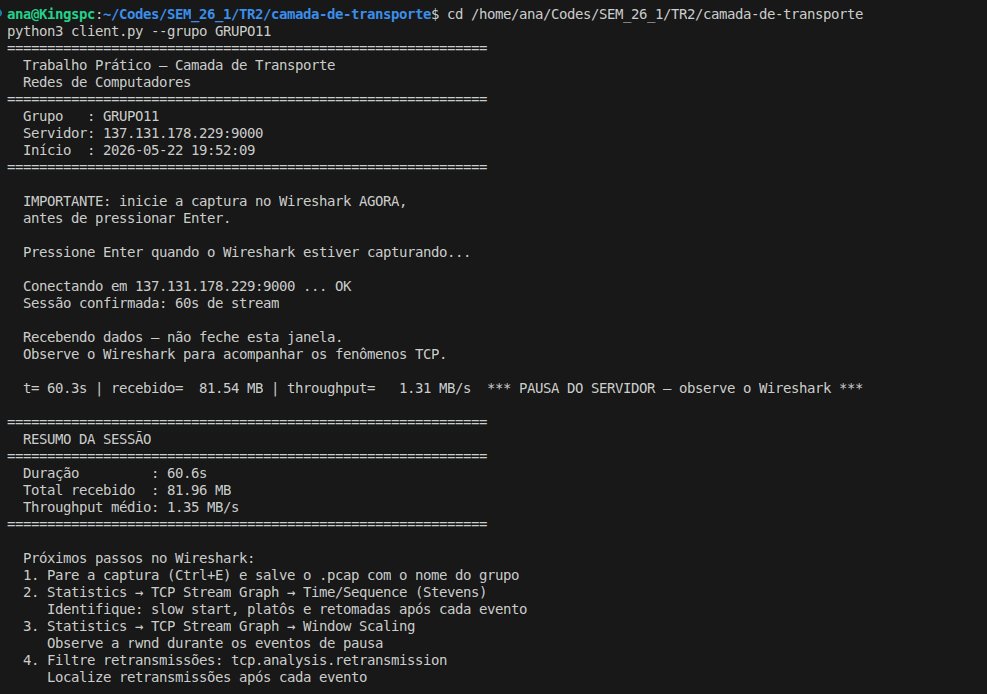
\includegraphics[width=0.9\textwidth]{captura/GRUPO11.png}
    \caption{Resumo da sessão exibido pelo terminal do cliente: duração 60,6 s,
    total recebido 81,96 MB e \textit{throughput} médio de 1,35 MB/s.}
    \label{fig:terminal}
\end{figure}

% ------------------------------------------------------------
% QUESTÃO 1
% ------------------------------------------------------------
\section{Questão 1 — Estabelecimento da Conexão e Parâmetros Iniciais}

\begin{figure}[H]
    \centering
    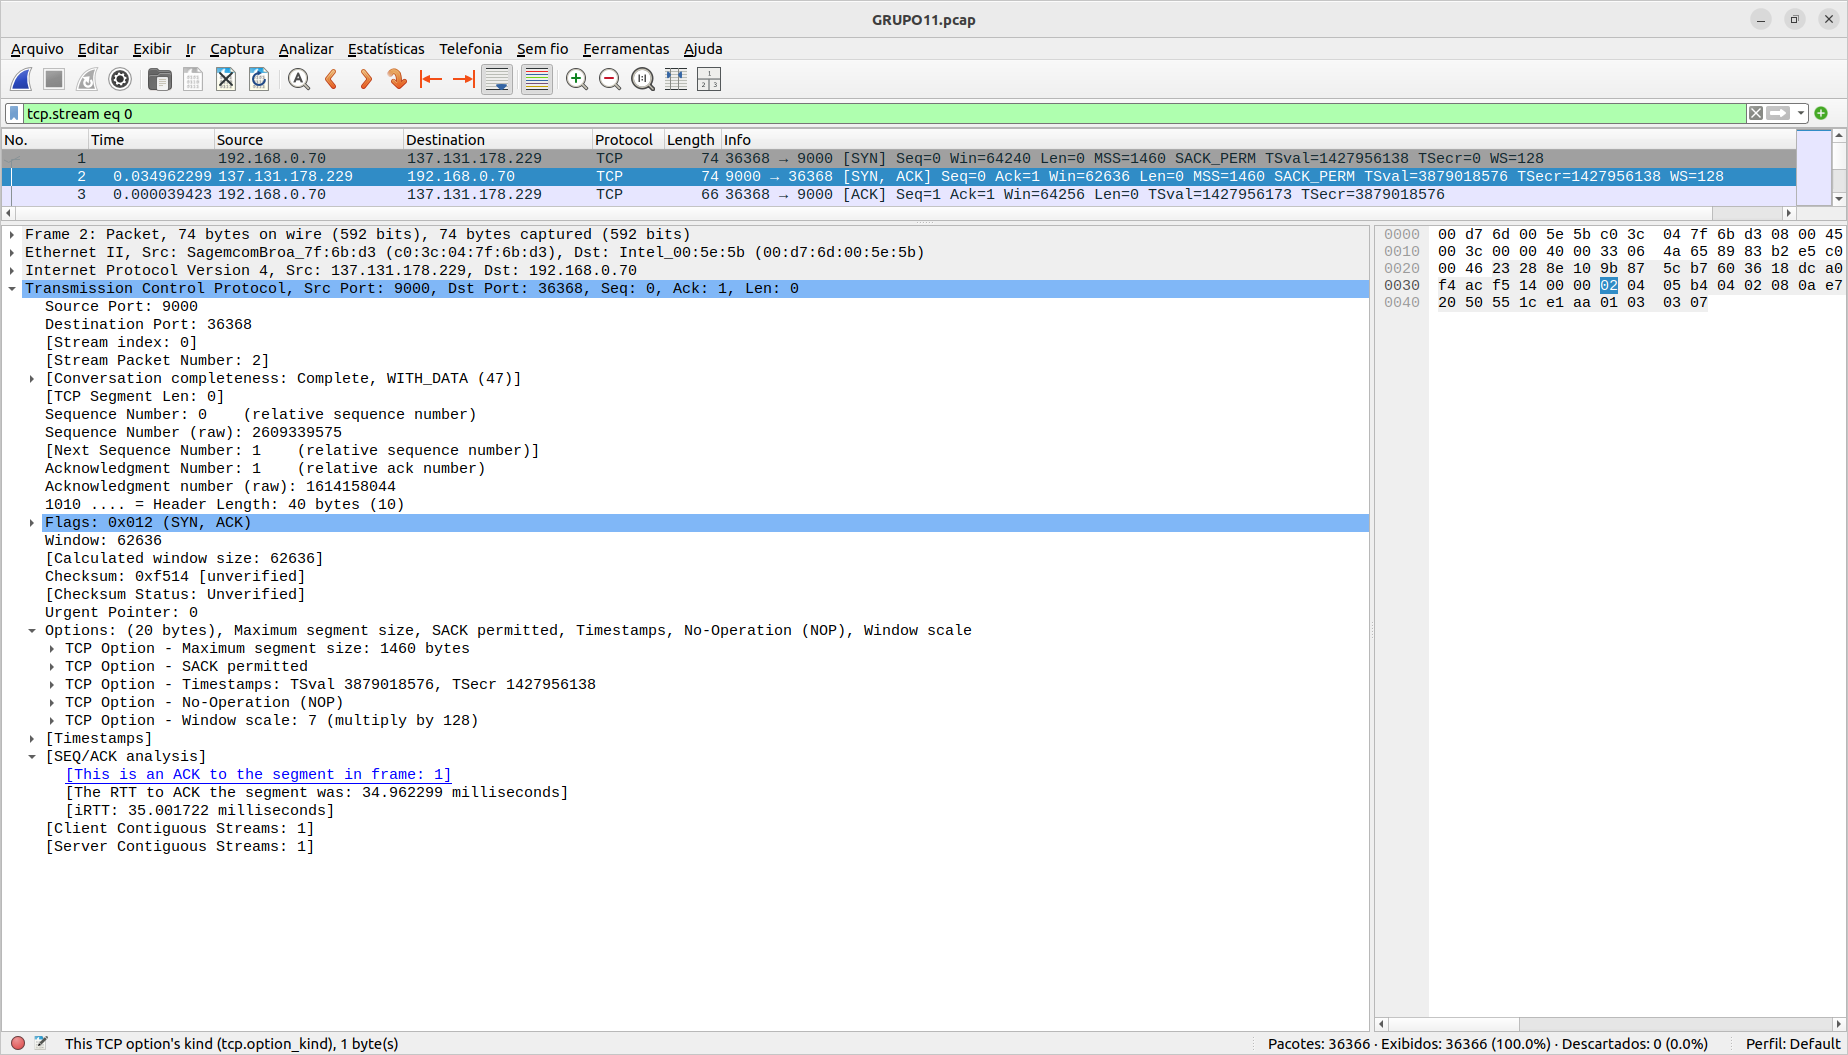
\includegraphics[width=\textwidth]{Q1/Q1.png}
    \caption{Lista de pacotes do Wireshark mostrando os três pacotes do \textit{handshake}
    (SYN, SYN-ACK, ACK) com os campos de RTT, MSS e janela expandidos no painel inferior.}
    \label{fig:q1}
\end{figure}

O \textit{three-way handshake} foi identificado no início da captura:

\begin{table}[H]
\centering
\begin{tabular}{@{}llll@{}}
    \toprule
    \textbf{Pacote} & \textbf{Timestamp} & \textbf{Flags} & \textbf{Sentido} \\
    \midrule
    SYN     & 19:52:15.002072 & \texttt{[S]}  & cliente $\to$ servidor \\
    SYN-ACK & 19:52:15.037034 & \texttt{[S.]} & servidor $\to$ cliente \\
    ACK     & 19:52:15.037074 & \texttt{[.]}  & cliente $\to$ servidor \\
    \bottomrule
\end{tabular}
\caption{Pacotes do \textit{three-way handshake} identificados na captura.}
\end{table}

\subsection*{(a) RTT entre SYN e SYN-ACK}
\textbf{34,962 ms.} Valor extraído do campo \texttt{[The RTT to ACK the segment was:
34.962299 milliseconds]}, visível em \texttt{[SEQ/ACK analysis]} do pacote SYN-ACK.

\subsection*{(b) MSS negociado}
\textbf{1460 bytes.} Cliente e servidor anunciaram MSS = 1460 bytes nas \textit{Options}
do SYN e do SYN-ACK; o MSS efetivo é o mínimo entre os dois, ou seja, 1460 bytes.

\subsection*{(c) Janela de recepção inicial (rwnd) no SYN-ACK}
\textbf{62.636 bytes.} Valor do campo \textit{Window Size Value} do SYN-ACK. O servidor
também negociou \textit{window scaling} com fator $\times 128$ (\texttt{wscale = 7}),
válido para os segmentos subsequentes; no próprio SYN-ACK, porém, o valor é o bruto,
sem escalonamento.

% ------------------------------------------------------------
% QUESTÃO 2
% ------------------------------------------------------------
\section{Questão 2 — Fluxo de Dados e Eventos de Pausa}

\begin{figure}[H]
    \centering
    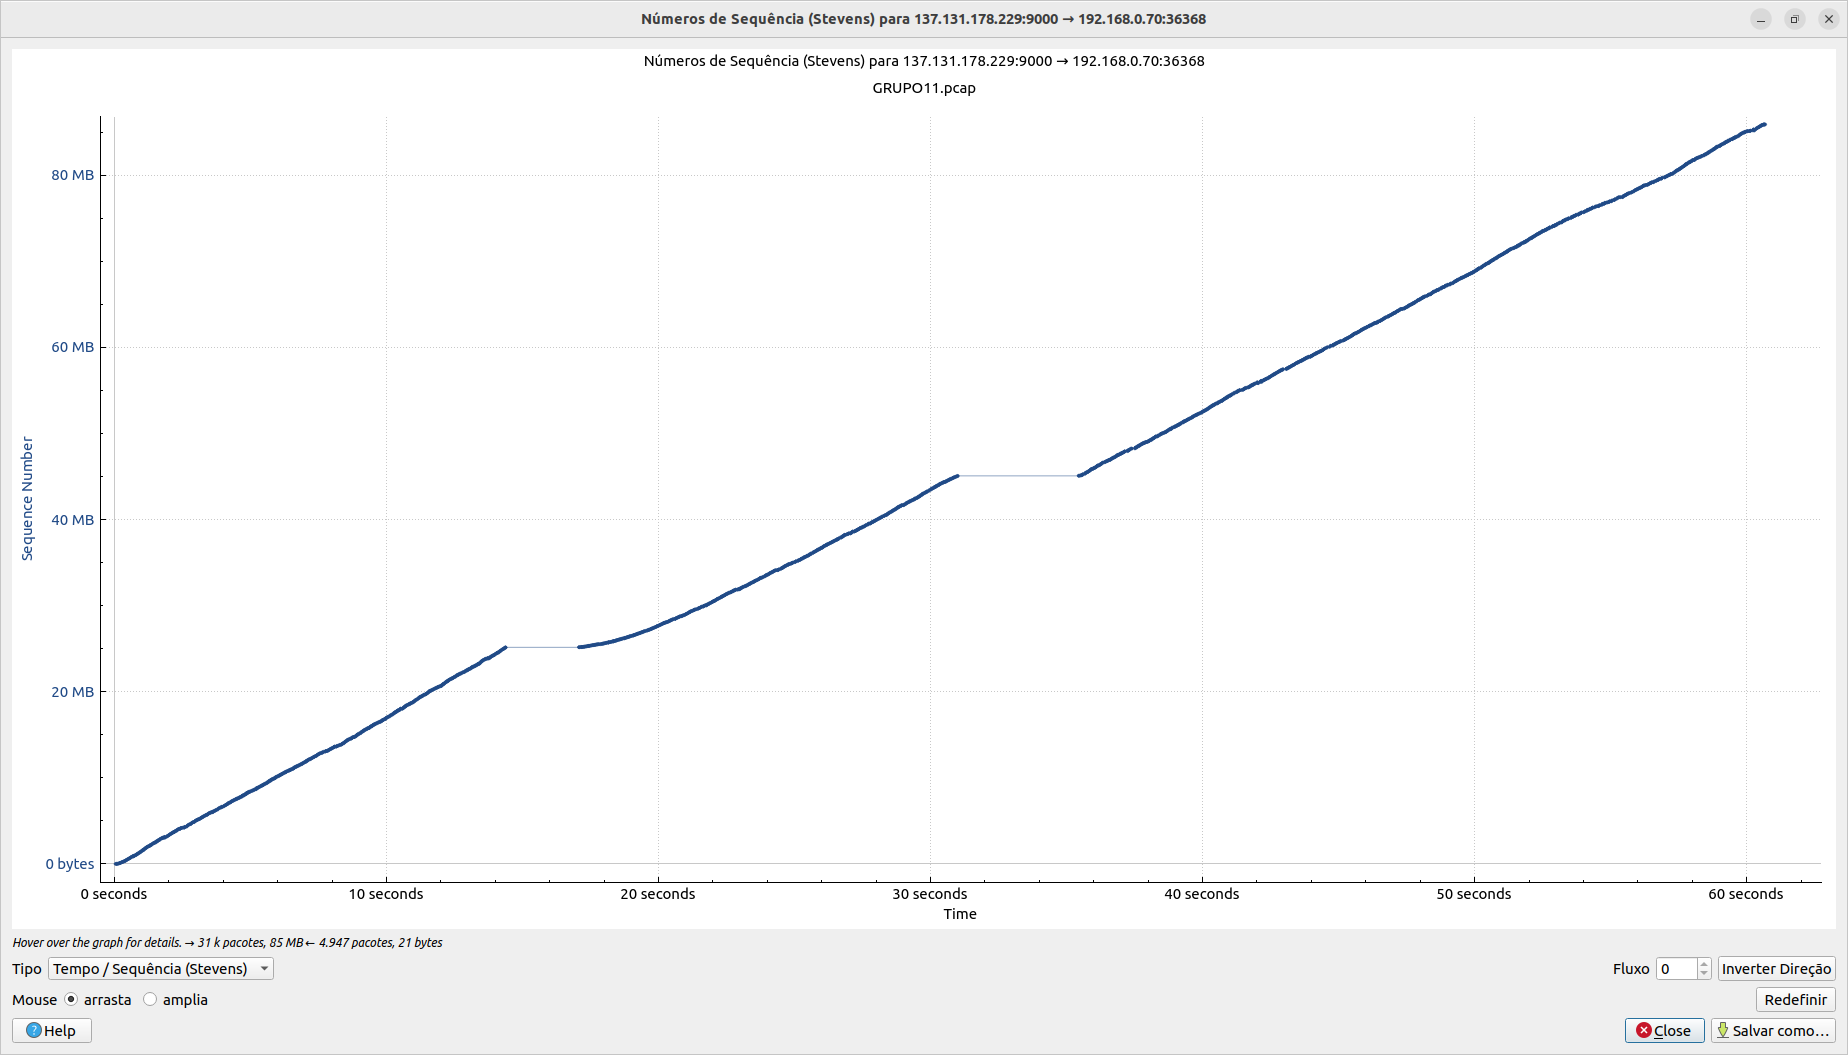
\includegraphics[width=0.95\textwidth]{Q2/Q2.png}
    \caption{Gráfico Time/Sequence (Stevens) — visão geral da sessão, com os dois platôs
    correspondentes às interrupções.}
    \label{fig:q2}
\end{figure}

O gráfico Stevens revelou \textbf{duas interrupções} no fluxo enviado pelo servidor,
visíveis como platôs horizontais:

\begin{table}[H]
\centering
\begin{tabular}{@{}lcc@{}}
    \toprule
     & \textbf{Interrupção 1} & \textbf{Interrupção 2} \\
    \midrule
    \textbf{(a) Início}             & 14,38 s & 31,00 s \\
    \textbf{(b) Bytes transferidos} & 25.163.380 B ($\approx$25,16 MB) & 45.087.444 B ($\approx$45,09 MB) \\
    \textbf{(c) Fim do platô}       & 17,08 s & 35,45 s \\
    \textbf{(c) Duração}            & \textbf{2,70 s} & \textbf{4,45 s} \\
    \bottomrule
\end{tabular}
\caption{Caracterização das duas interrupções no gráfico Stevens.}
\end{table}

O \textbf{início} de cada interrupção corresponde ao instante em que a curva de números
de sequência deixa de crescer e se torna horizontal; o \textbf{fim}, ao ponto em que a
curva volta a subir. Esse comportamento é característico de pausa no lado do servidor,
e não de perda de pacotes isolados.

\begin{figure}[H]
    \centering
    \begin{minipage}{0.48\textwidth}
        \centering
        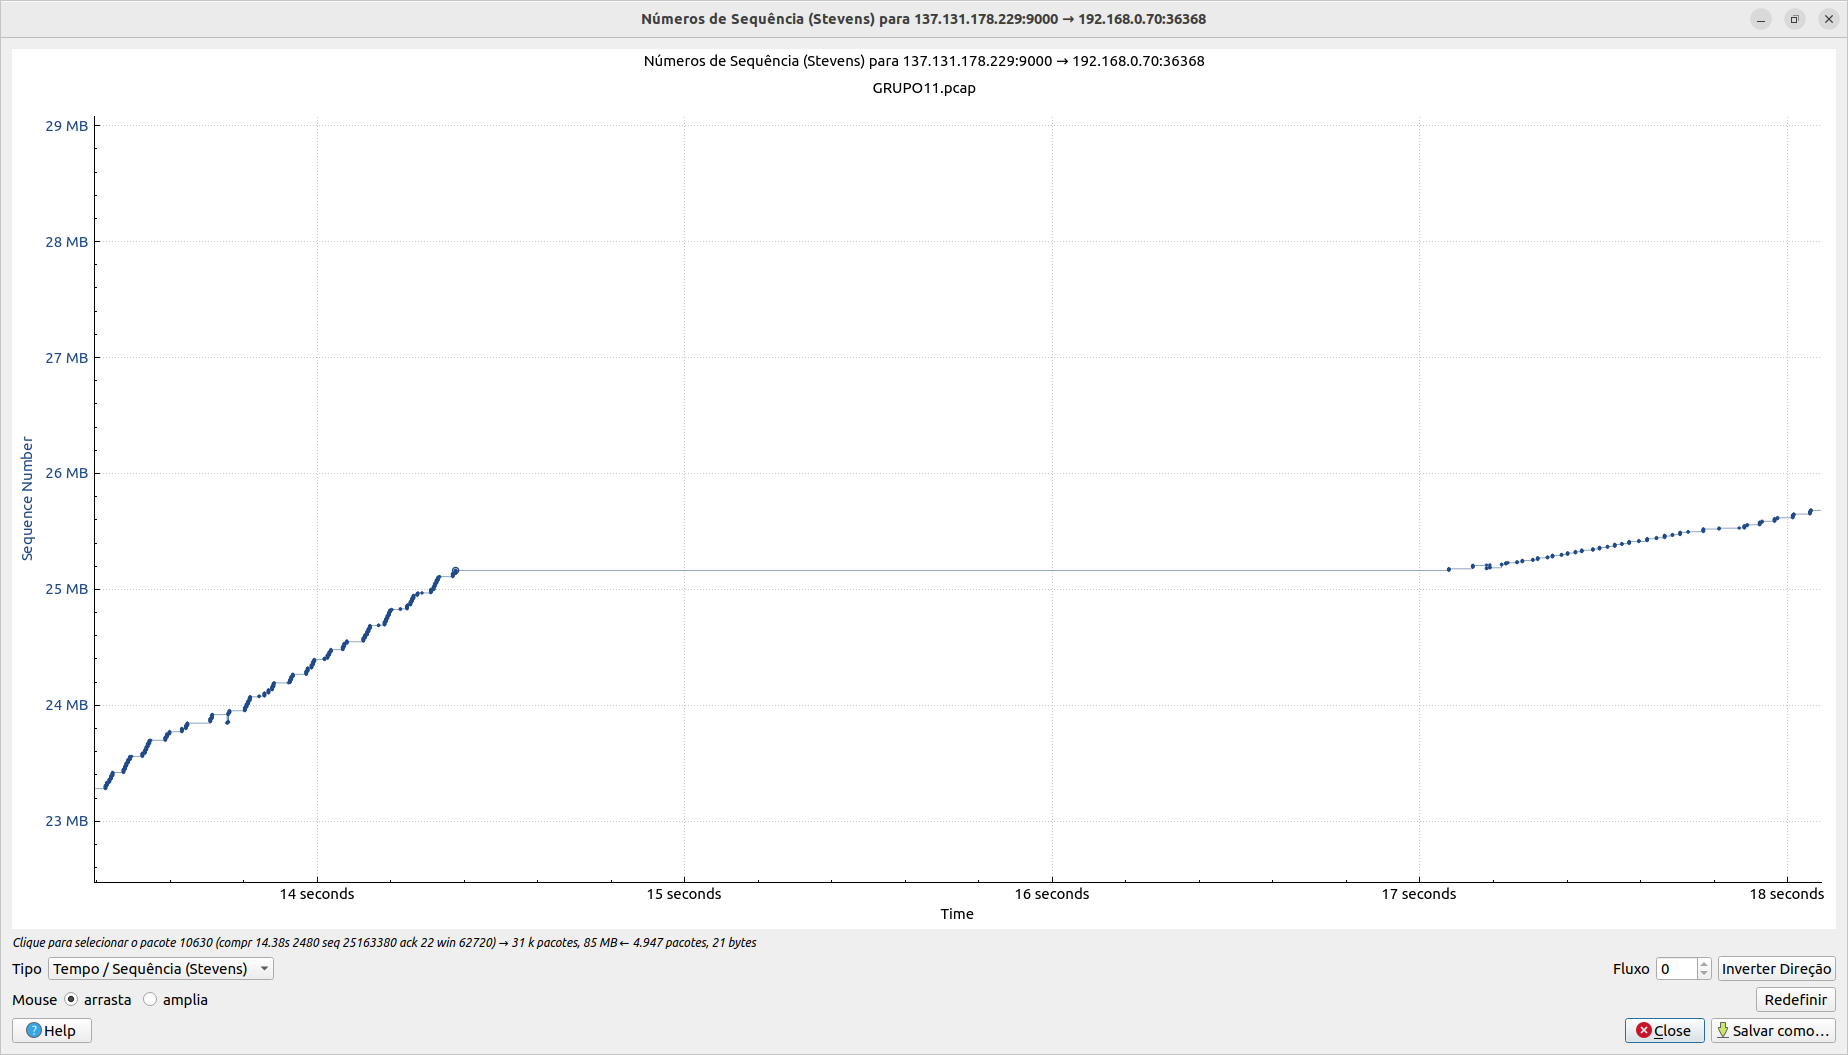
\includegraphics[width=\textwidth]{Q2/Q2_1.png}
        \caption{Interrupção 1 — início ($\approx$14,38 s)}
    \end{minipage}
    \hfill
    \begin{minipage}{0.48\textwidth}
        \centering
        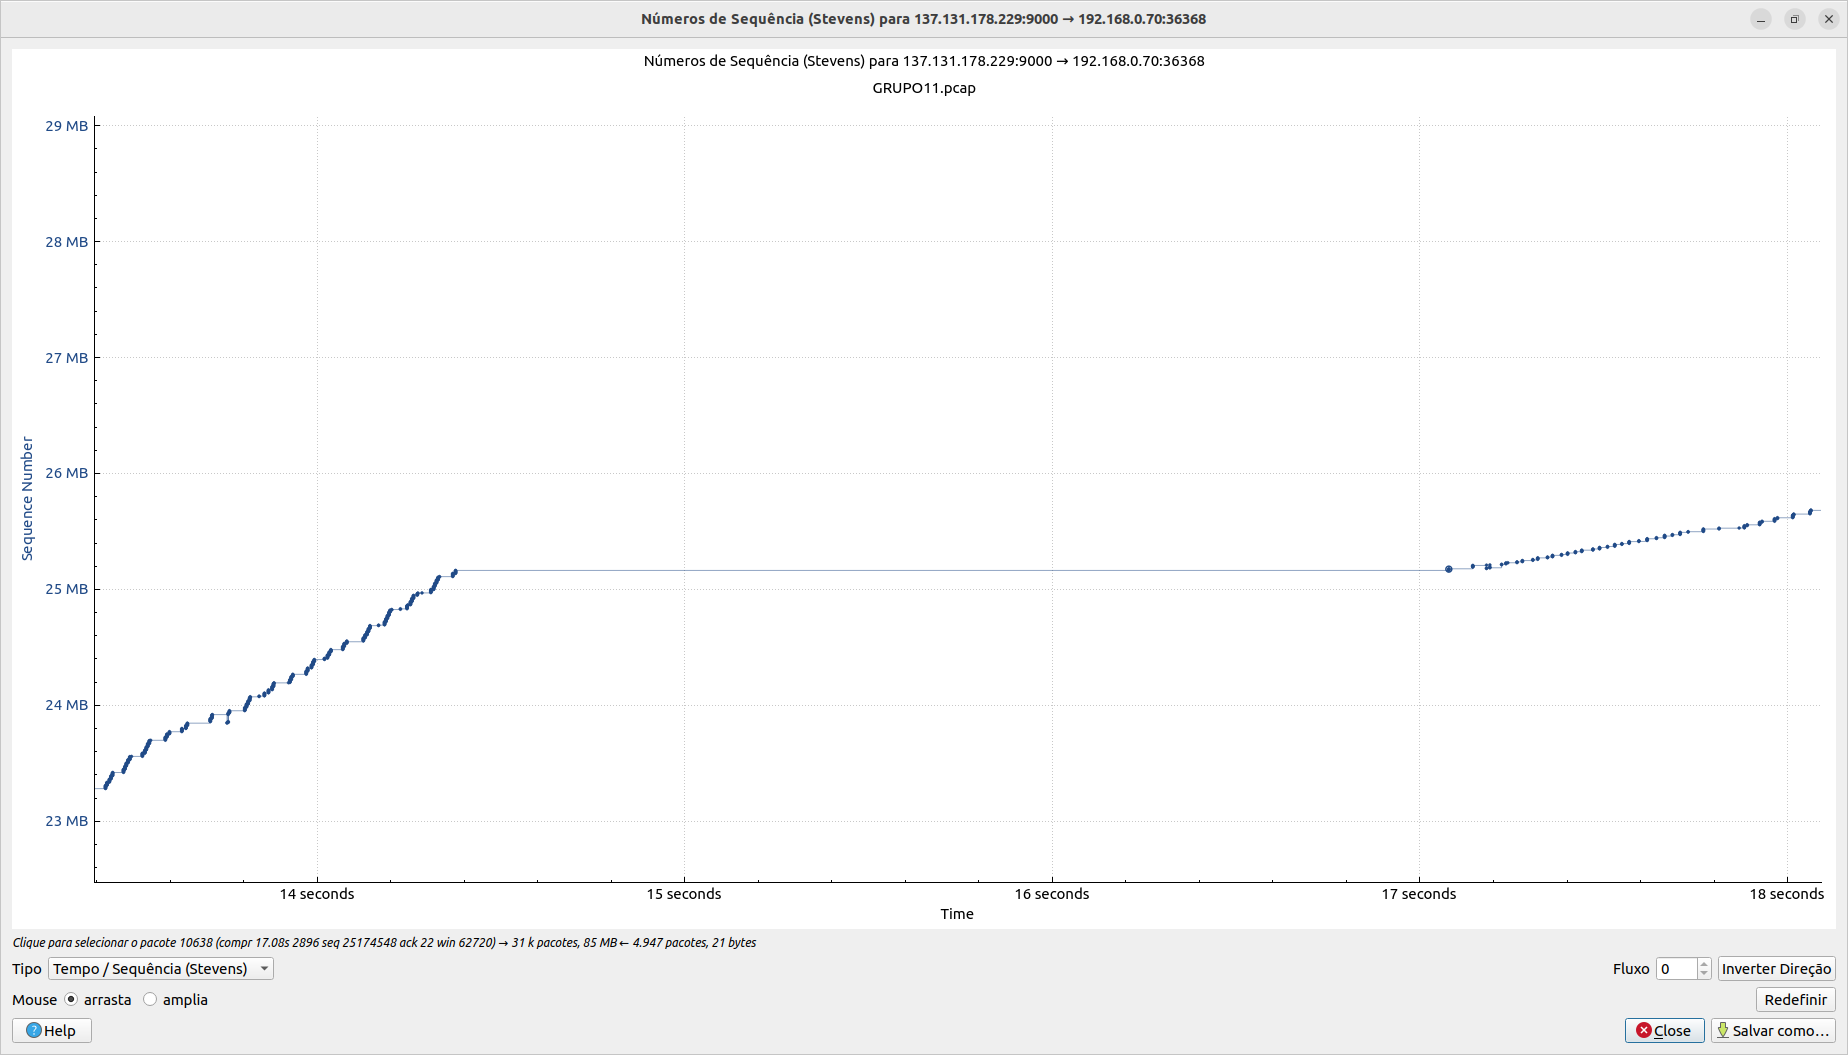
\includegraphics[width=\textwidth]{Q2/Q2_2.png}
        \caption{Interrupção 1 — fim do platô ($\approx$17,08 s)}
    \end{minipage}
\end{figure}

\begin{figure}[H]
    \centering
    \begin{minipage}{0.48\textwidth}
        \centering
        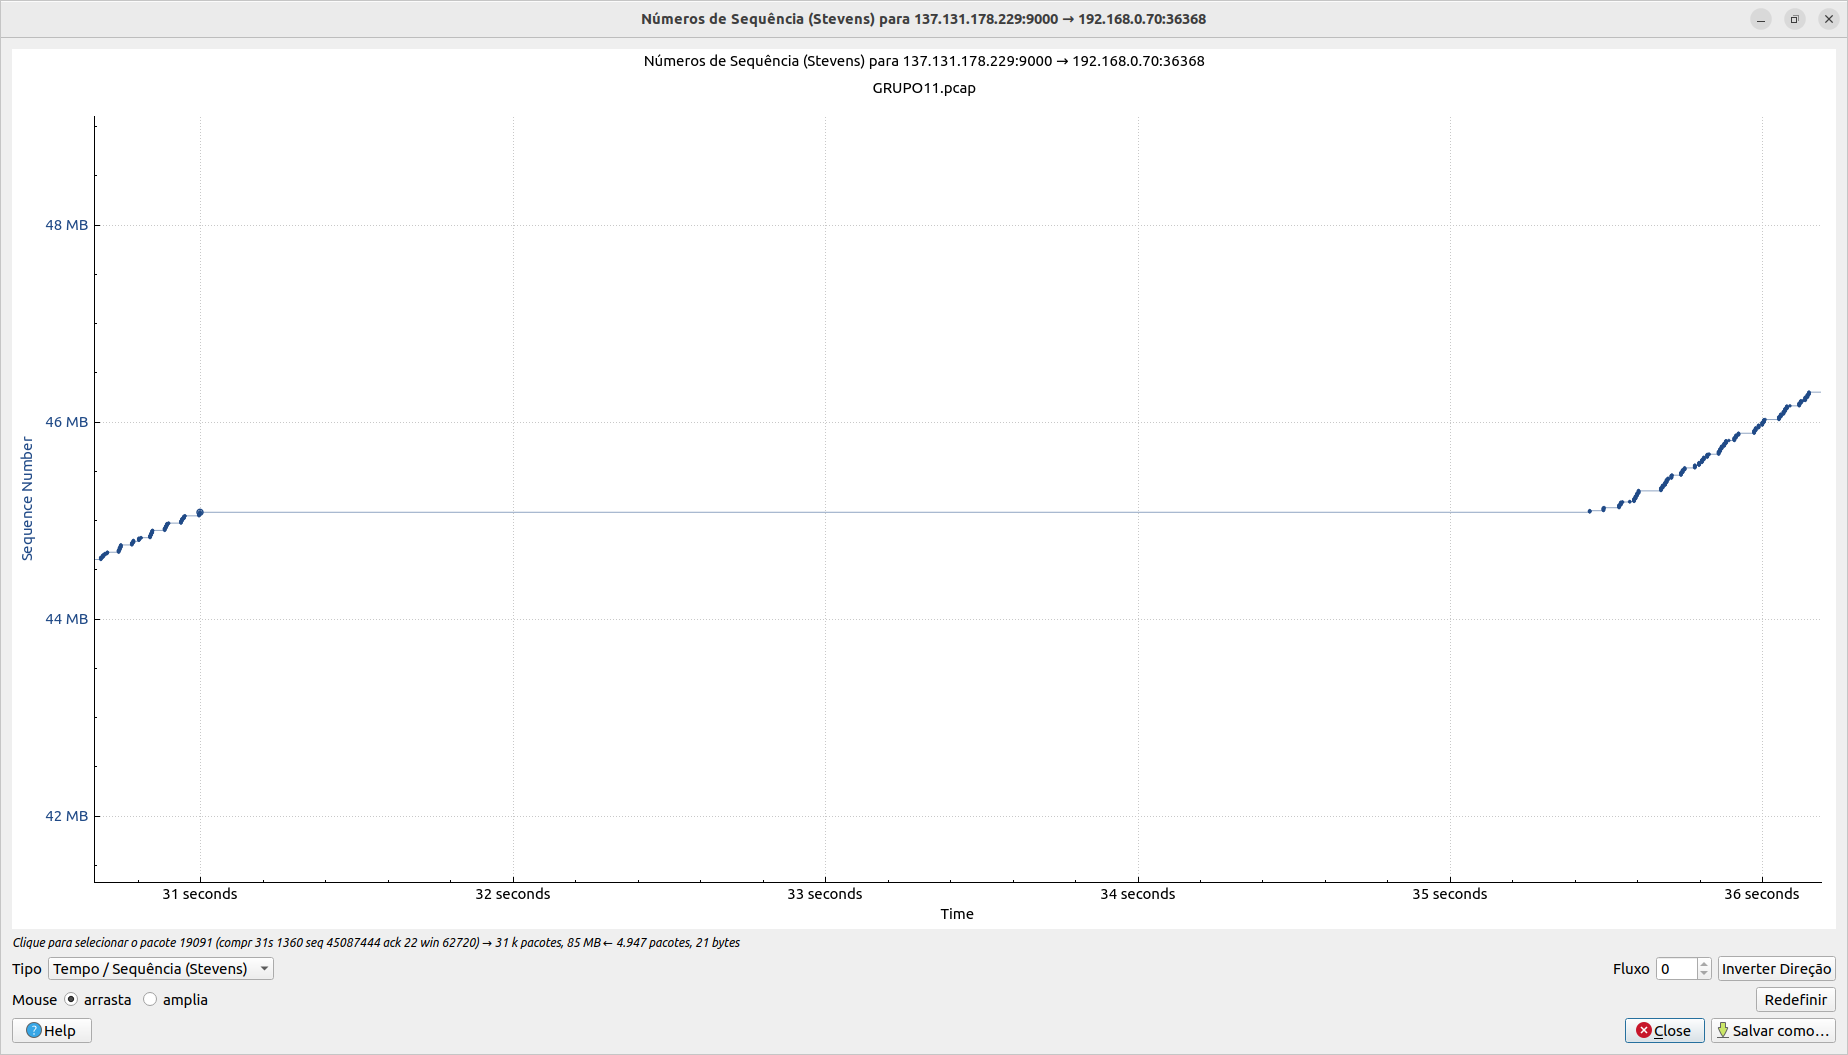
\includegraphics[width=\textwidth]{Q2/Q2_3.png}
        \caption{Interrupção 2 — início ($\approx$31,00 s)}
    \end{minipage}
    \hfill
    \begin{minipage}{0.48\textwidth}
        \centering
        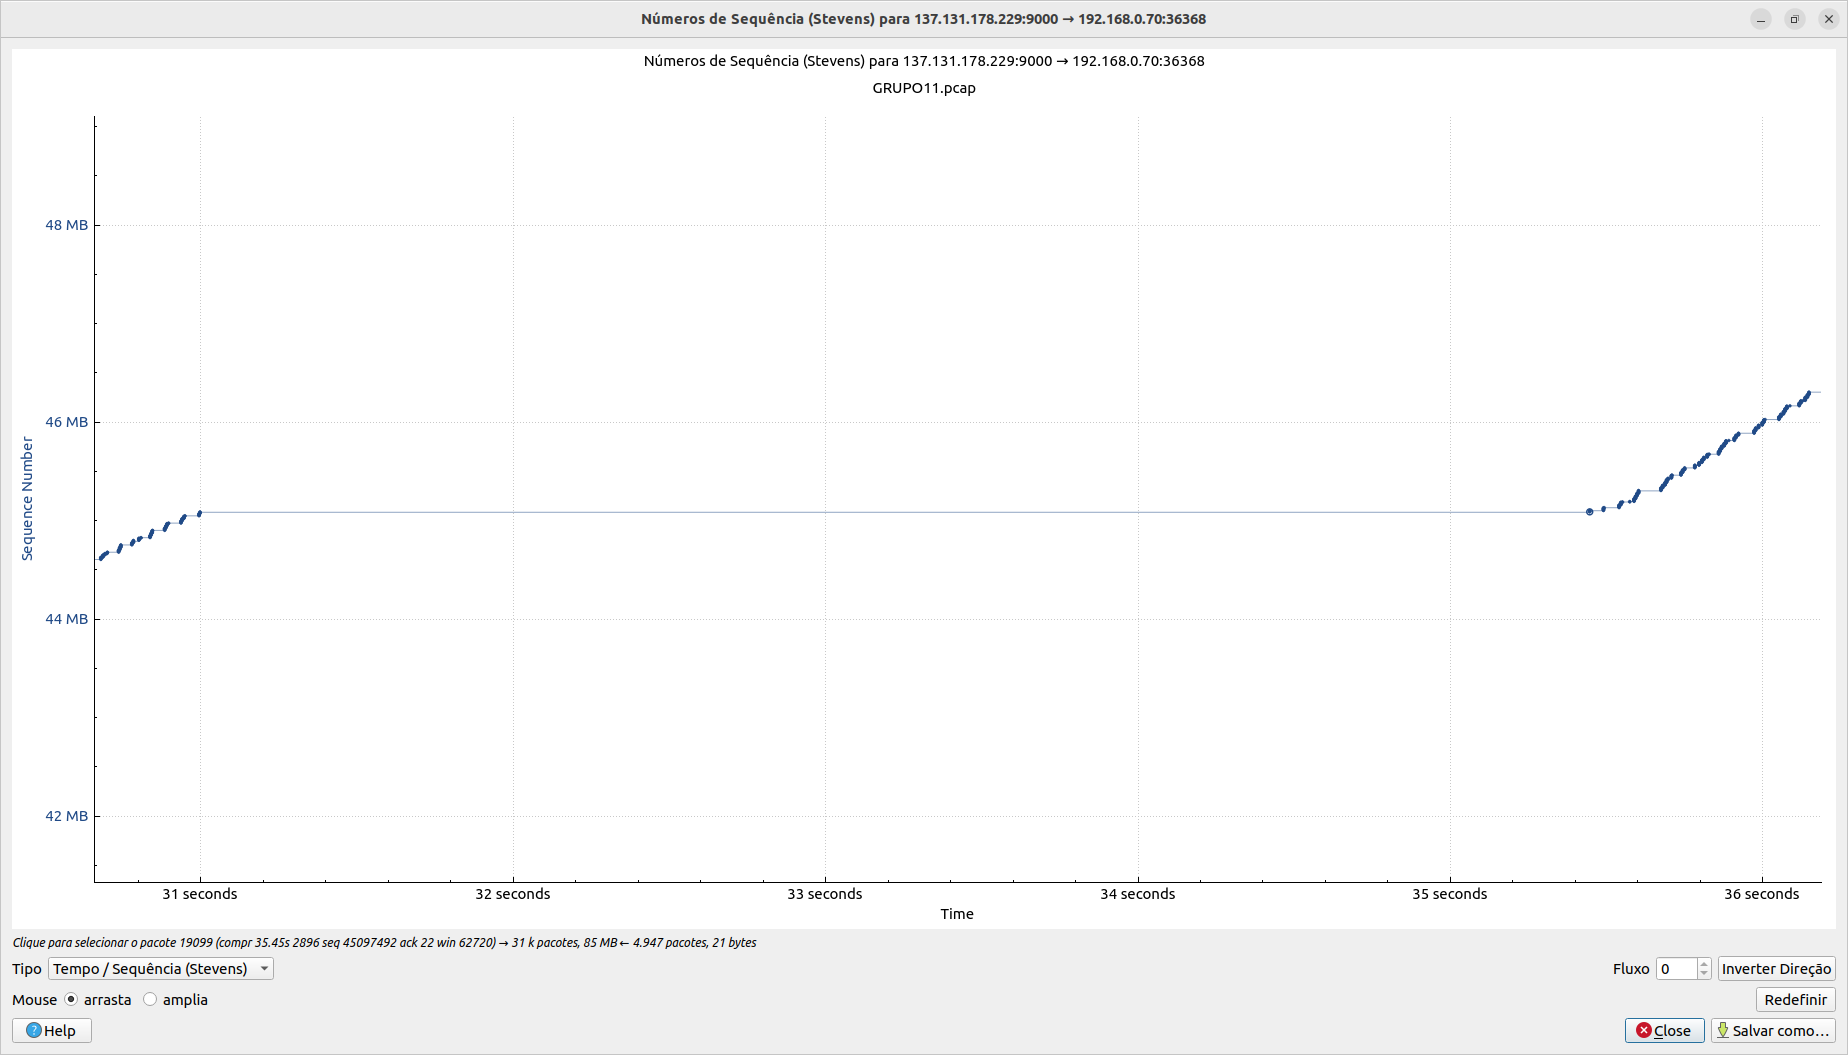
\includegraphics[width=\textwidth]{Q2/Q2_4.png}
        \caption{Interrupção 2 — fim do platô ($\approx$35,45 s)}
    \end{minipage}
\end{figure}

% ------------------------------------------------------------
% QUESTÃO 3
% ------------------------------------------------------------
\section{Questão 3 — Algoritmo de Controle de Congestionamento}

O algoritmo de controle de congestionamento em uso na máquina é o \textbf{\texttt{cubic}}
(padrão do Linux), confirmado pelo comando \texttt{Get-NetTCPSetting | Select CongestionProvider}
(Figura~\ref{fig:q3cmd}).

\begin{figure}[H]
    \centering
    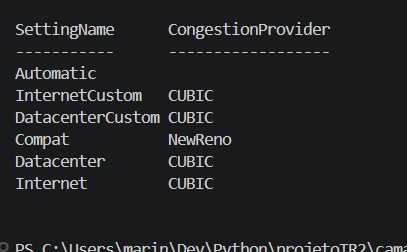
\includegraphics[width=0.65\textwidth]{Q3/Q3_command.png}
    \caption{Configuração do algoritmo de controle de congestionamento TCP — CUBIC.}
    \label{fig:q3cmd}
\end{figure}

\begin{figure}[H]
    \centering
    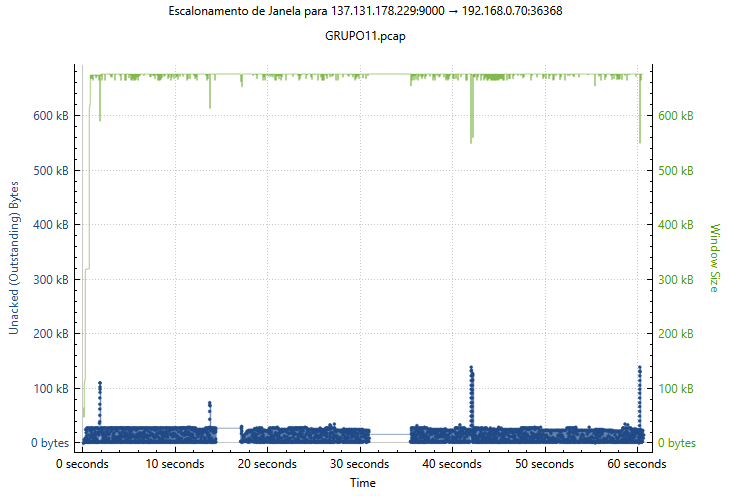
\includegraphics[width=0.95\textwidth]{Q3/Q3.png}
    \caption{Gráfico Window Scaling com as curvas \textit{Bytes Out} (bytes em voo)
    e \textit{Rcv Win} (janela de recepção) ao longo de toda a sessão.}
    \label{fig:q3}
\end{figure}

\begin{figure}[H]
    \centering
    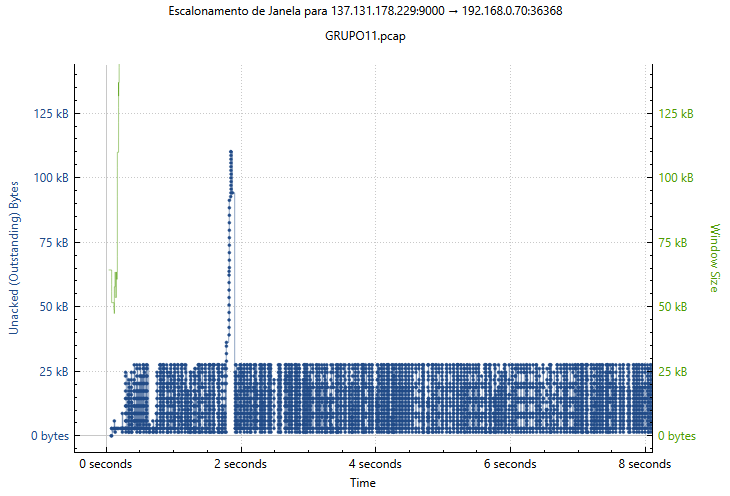
\includegraphics[width=0.95\textwidth]{Q3/Zoom_Intervalo_0_2s.png}
    \caption{Zoom no intervalo 0--2 s: crescimento exponencial de \textit{Bytes Out},
    evidenciando a fase de \textit{Slow Start}.}
    \label{fig:q3zoom}
\end{figure}

\subsection*{(a) Bytes Out nos primeiros segundos}
Nos primeiros $\approx$2 segundos, a curva \textit{Bytes Out} cresce de forma exponencial
acentuada --- comportamento típico da fase de \textbf{Slow Start}, em que a \textit{cwnd}
aproximadamente dobra a cada RTT para ocupar rapidamente a banda disponível.

\subsection*{(b) Bytes Out e Rcv Win durante as interrupções}
Nas duas interrupções, a curva \textit{Bytes Out} \textbf{desaba para zero}: o servidor
para de enviar e os ACKs pendentes continuam chegando. A \textit{Rcv Win} anunciada pelo
cliente \textbf{permanece alta e estável}, comprovando que as pausas foram causadas pelo
\textbf{servidor} e não por controle de fluxo do receptor.

\subsection*{(c) Retomada após cada interrupção}
A retomada de \textit{Bytes Out} é \textbf{abrupta e quase vertical}. Como não houve
perda real (apenas pausa de aplicação), o TCP pôde reatar de forma agressiva, preservando
as métricas anteriores da conexão.

\subsection*{(d) Consistência com o Kurose (Cap.\ 3)}
O comportamento é consistente com a teoria: a fase inicial reproduz o \textit{Slow Start}
clássico. A queda a zero e a retomada imediata confirmam que o \textbf{TCP CUBIC} trata
\textit{application stalls} de modo diferenciado: como não houve \textit{timeouts} por
perda, o \textit{ssthresh} não foi derrubado, permitindo reativação muito mais rápida
do que o TCP Reno clássico faria.

% ------------------------------------------------------------
% QUESTÃO 4
% ------------------------------------------------------------
\section{Questão 4 — Retransmissões, ACKs Duplicados e SACK}

\begin{figure}[H]
    \centering
    \begin{minipage}{0.48\textwidth}
        \centering
        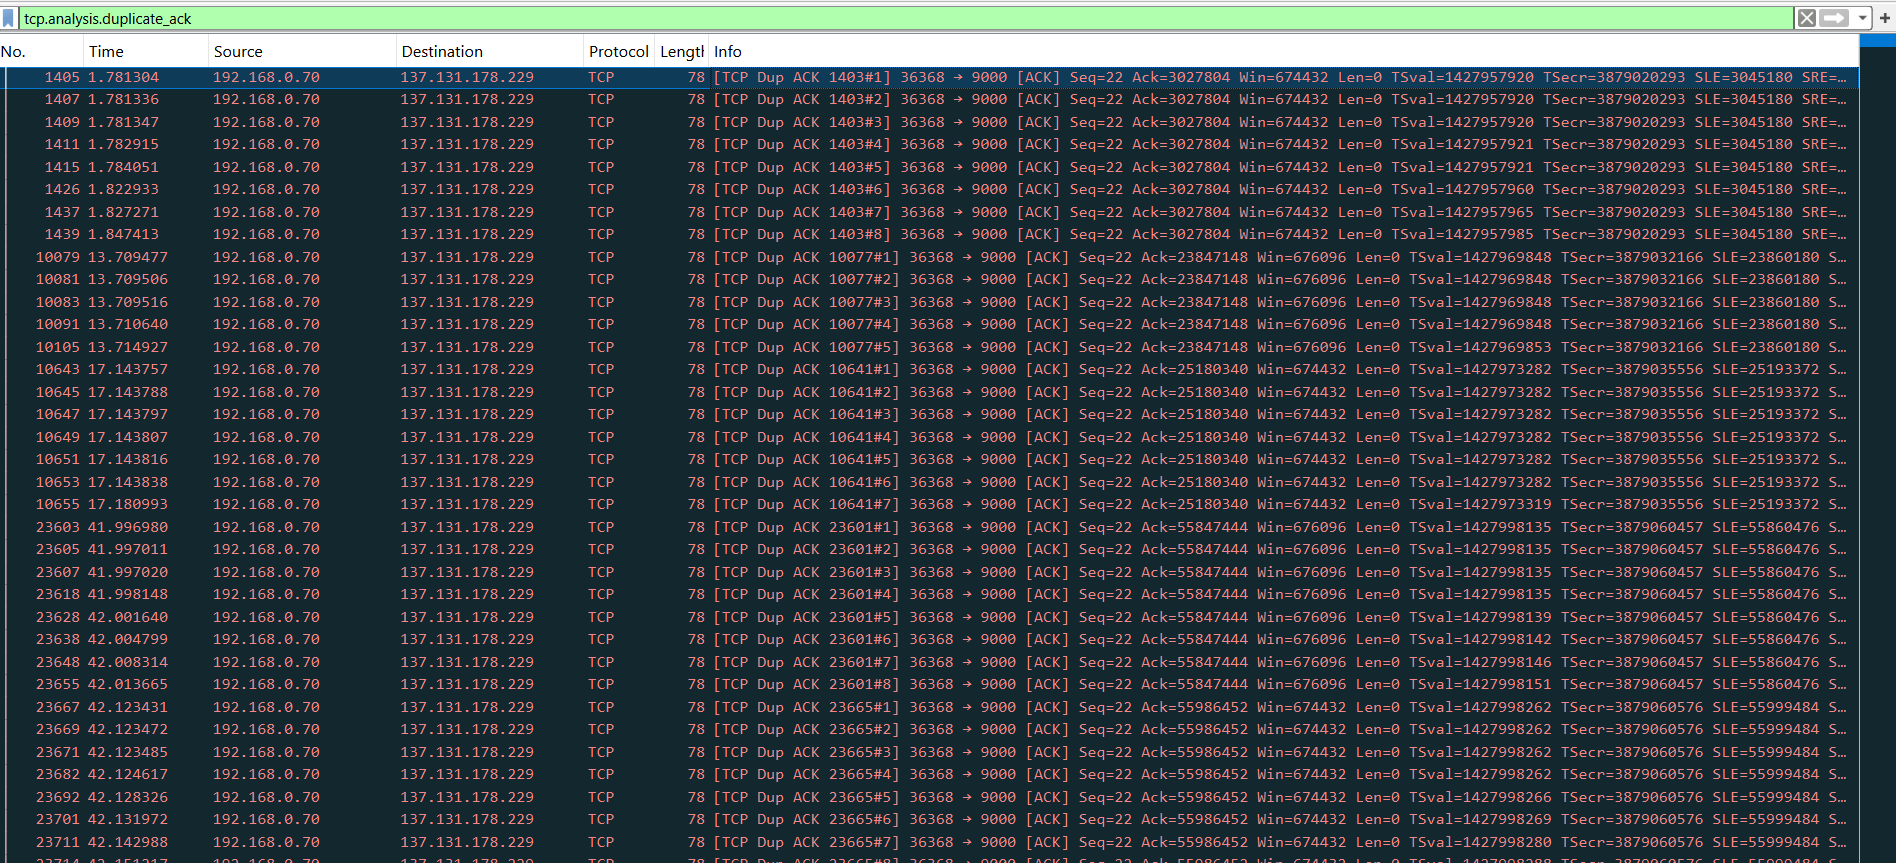
\includegraphics[width=\textwidth]{Q4/ack_duplicados1.png}
        \caption{Filtro \texttt{tcp.analysis.duplicate\_ack} — visão geral}
    \end{minipage}
    \hfill
    \begin{minipage}{0.48\textwidth}
        \centering
        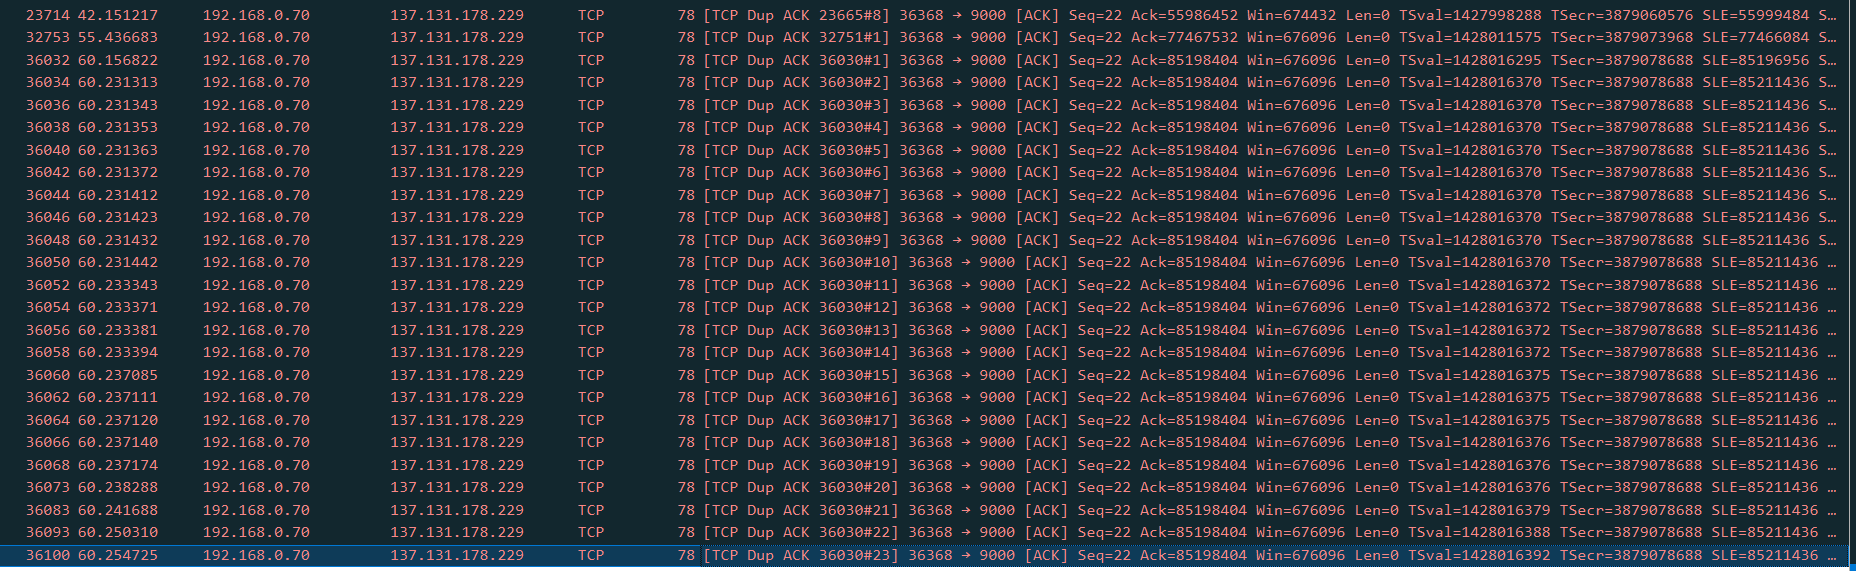
\includegraphics[width=\textwidth]{Q4/ack_duplicados2.png}
        \caption{Filtro \texttt{tcp.analysis.duplicate\_ack} — sequência \#23}
    \end{minipage}
\end{figure}

\begin{figure}[H]
    \centering
    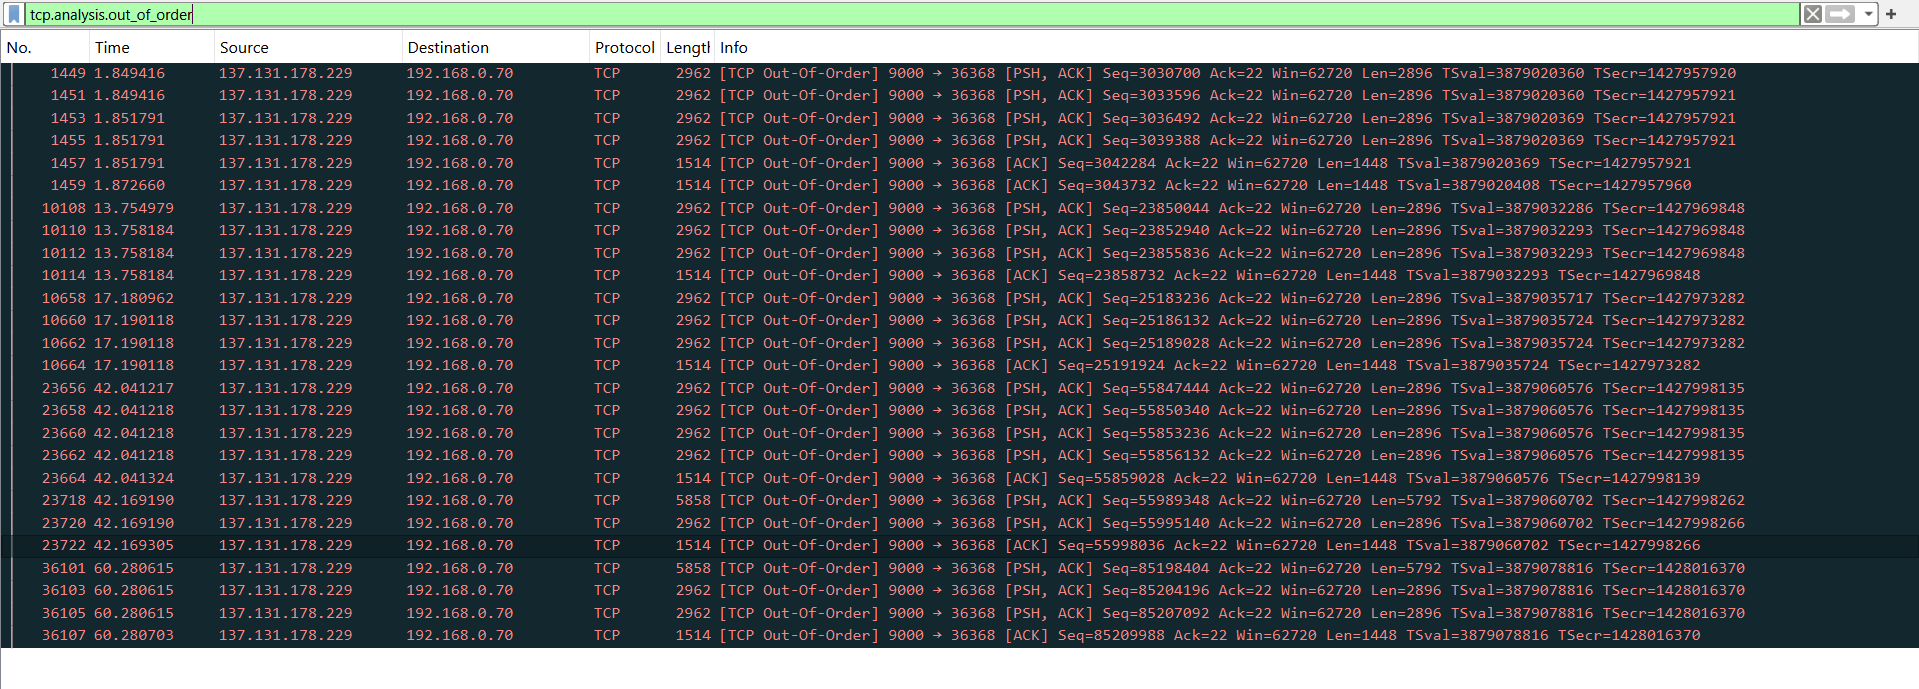
\includegraphics[width=0.95\textwidth]{Q4/acks_foraDeOrdem.png}
    \caption{Filtro \texttt{tcp.analysis.out\_of\_order}: pacotes entregues fora de ordem.}
    \label{fig:q4ooo}
\end{figure}

\begin{figure}[H]
    \centering
    \begin{minipage}{0.48\textwidth}
        \centering
        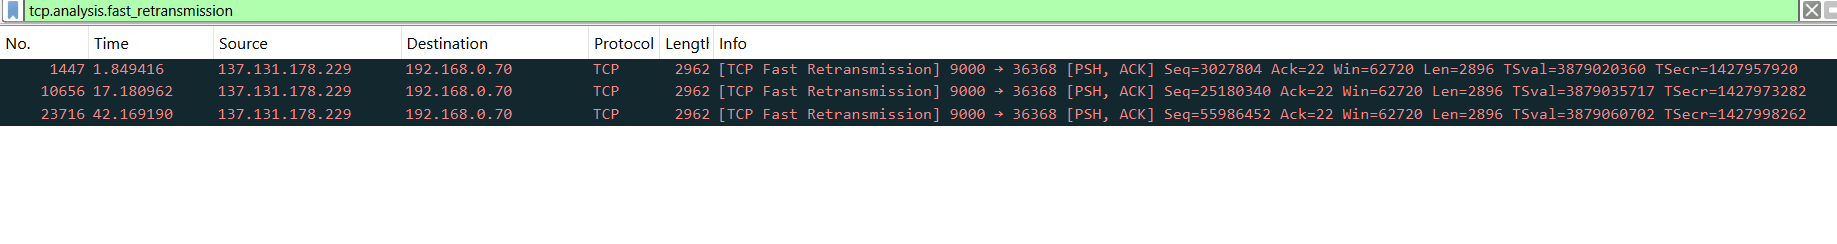
\includegraphics[width=\textwidth]{Q4/fast_retransmition.png}
        \caption{Filtro \texttt{tcp.analysis.fast\_retransmission}}
    \end{minipage}
    \hfill
    \begin{minipage}{0.48\textwidth}
        \centering
        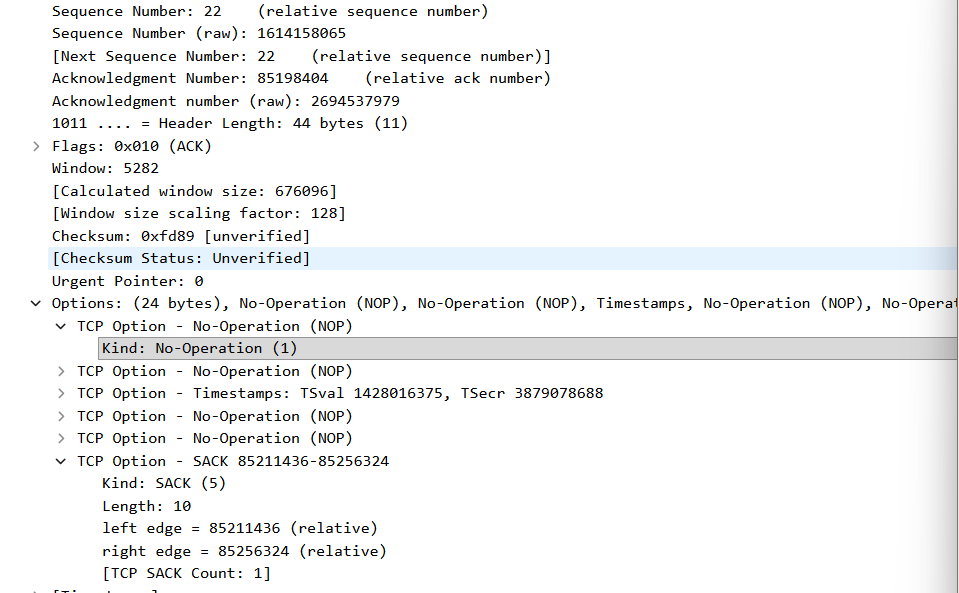
\includegraphics[width=\textwidth]{Q4/sack_expandido.png}
        \caption{Bloco SACK expandido com Left/Right Edge}
    \end{minipage}
\end{figure}

\subsection*{(a) Filtro \texttt{tcp.analysis.duplicate\_ack}}
Foram detectados \textbf{60 ACKs duplicados}. A maior sequência consecutiva foi
\texttt{[TCP Dup ACK 36030\#23]} (Frame \#36100): o cliente reenviou o mesmo aviso
\textbf{23 vezes seguidas}. O \textit{Acknowledgment Number} exigido foi
\textbf{85.198.404} ($\approx$85,19 MB), indicando que o fluxo travou aguardando esse
byte para avançar a janela de recepção.

\subsection*{(b) Filtro \texttt{tcp.analysis.out\_of\_order}}
Foram detectados \textbf{26 pacotes fora de ordem}. Distinção visual no Wireshark:
\begin{itemize}[leftmargin=1.4em, itemsep=2pt]
    \item \textbf{Out-of-order:} segmento que chega com número de sequência menor que o
    maior já registrado, dentro de $\approx$1 RTT — buraco preenchido logo em seguida.
    Indica apenas caminhos/atrasos diferentes, sem descarte.
    \item \textbf{Perda real:} sinalizada por sequência \textit{persistente} de DupACKs,
    encerrada por um pacote classificado como \texttt{[TCP Fast Retransmission]}.
\end{itemize}

\subsection*{(c) Filtro \texttt{tcp.analysis.fast\_retransmission}}
Ocorreram \textbf{3 \textit{fast retransmissions}}. O SACK estava habilitado (negociado
no \textit{handshake}). Foi identificado \textbf{1 bloco SACK} com:
\begin{itemize}[leftmargin=1.4em, itemsep=2pt]
    \item \textbf{Left Edge:} \texttt{85.211.436}
    \item \textbf{Right Edge:} \texttt{85.256.324}
\end{itemize}
Essas extremidades informam ao servidor que os bytes nesse intervalo já chegaram ao
cliente, de modo que ele retransmita \textit{apenas} o segmento ausente (a partir do byte
85.198.404), sem reenviar o bloco já recebido.

\subsection*{(d) Fast Retransmit ou Timeout?}
Todas as retransmissões foram disparadas por \textbf{Fast Retransmit}. O servidor não
esperou o estouro do temporizador: ao receber o limiar de \textbf{3 ACKs duplicados} ---
chegando a 23 notificações consecutivas no caso mais crítico --- assumiu a perda e
reenviou imediatamente.

% ------------------------------------------------------------
% QUESTÃO 5
% ------------------------------------------------------------
\section{Questão 5 — Vazão, Goodput e Overhead de Protocolo}

\begin{figure}[H]
    \centering
    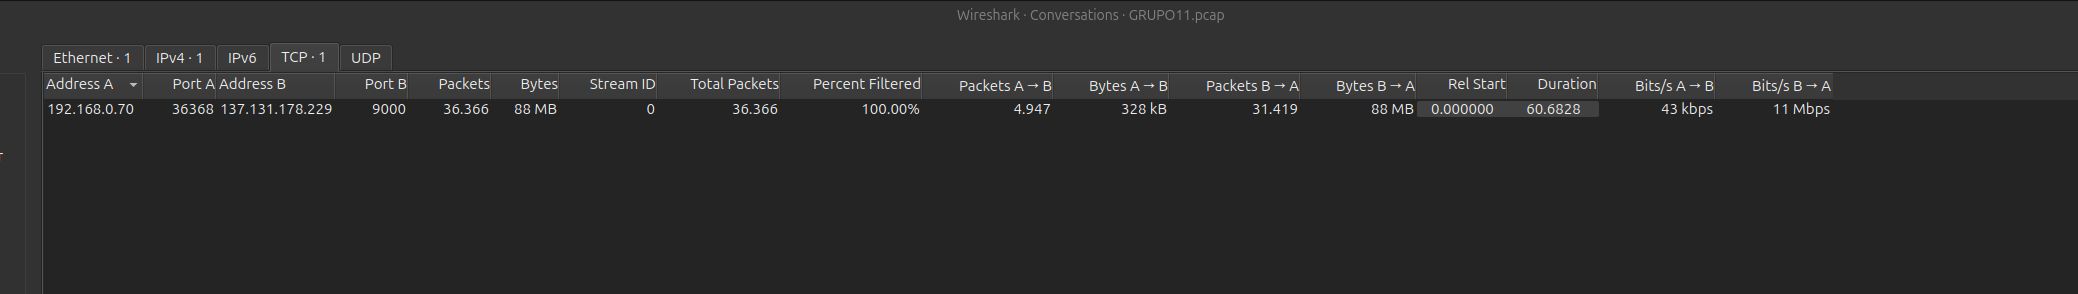
\includegraphics[width=0.95\textwidth]{Q5/Q5_conversations.png}
    \caption{Statistics $\to$ Conversations (aba TCP): 31.419 pacotes e $\approx$88 MB
    de servidor para cliente; Bits/s B$\to$A $\approx$11 Mbps.}
    \label{fig:q5conv}
\end{figure}

\begin{figure}[H]
    \centering
    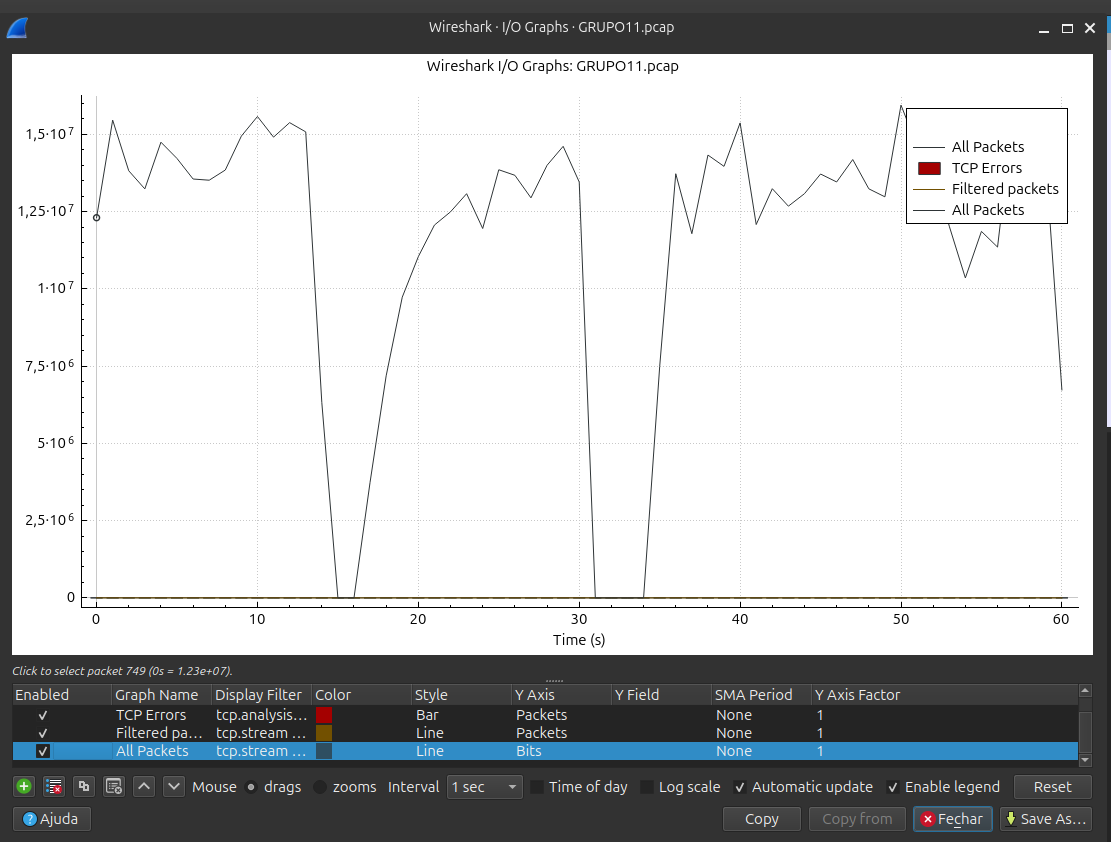
\includegraphics[width=0.95\textwidth]{Q5/Q5_iograph.png}
    \caption{Statistics $\to$ IO Graph com filtro \texttt{tcp.stream eq 0} em Bits/s.
    As duas quedas a zero coincidem com as interrupções das Questões 2 e 3.}
    \label{fig:q5io}
\end{figure}

\subsection*{(a) O valor reportado pelo cliente é goodput ou throughput?}
O cliente reportou \textbf{81,96 MB} recebidos e \textit{throughput} médio de
\textbf{1,35 MB/s} ($\approx$11,3 Mbps). Esse valor é \textbf{goodput}. O cliente acumula
\texttt{total += len(data)} a cada \texttt{sock.recv()}, que entrega à aplicação apenas o
payload TCP, em ordem e sem duplicatas, sem contar cabeçalhos nem bytes retransmitidos.

\subsection*{(b) Vazão do mesmo stream no Wireshark}
\textbf{Statistics $\to$ Conversations (aba TCP)}: Bytes B$\to$A $\approx$\textbf{88 MB};
Bits/s B$\to$A $\approx$\textbf{11 Mbps}; Duração: 60,68 s.\\[4pt]
\textbf{Statistics $\to$ IO Graph} com \texttt{tcp.stream eq 0} em Bits/s: vazão média
$\approx$\textbf{11,5 Mbps}, com duas quedas a zero em $\approx$15 s e $\approx$31--34 s.
Ambas medem \textbf{throughput bruto} e incluem cabeçalhos e retransmissões.

\subsection*{(c) Comparação cliente $\times$ Wireshark}

\begin{table}[H]
\centering
\begin{tabular}{@{}lcc@{}}
    \toprule
    \textbf{Medida} & \textbf{Valor} & \textbf{Inclui cabeçalhos/retx?} \\
    \midrule
    Cliente (goodput)    & 1,35 MB/s $\approx$ \textbf{11,3 Mbps} & Não \\
    Wireshark (nível IP) & 1,376 MB/s $\approx$ \textbf{11,5 Mbps} & Sim \\
    Wireshark (frame)    & 1,383 MB/s $\approx$ \textbf{11,6 Mbps} & Sim \\
    \bottomrule
\end{tabular}
\caption{Comparação entre goodput do cliente e throughput bruto do Wireshark.}
\end{table}

Os valores \textbf{não são iguais}: o do Wireshark é \textbf{maior}, pois inclui o
overhead dos cabeçalhos e as retransmissões.

\subsection*{(d) Overhead percentual: esperado vs.\ observado}

Cálculo manual (cabeçalhos IP + TCP = 20 + 20 = 40 B sobre 1390 B de payload):
\begin{equation*}
\text{overhead}\,(\%) = \frac{40}{1390 + 40} \times 100 = \mathbf{2{,}80}\,\%
\end{equation*}

\textbf{Observado na captura:} 1,87\,\% (nível IP) e 2,36\,\% (nível de frame). O resultado
está na mesma faixa dos 2,80\,\% teóricos. A diferença ficou ligeiramente abaixo porque a
placa de rede usou \textit{segmentation offload} (LRO/GRO): o payload médio por frame
capturado foi de \textbf{2.736 bytes} ($\approx$2 segmentos coalescidos), registrando
menos cabeçalhos no trace do que existiriam no fio físico.

\begin{table}[H]
\centering
\begin{tabular}{@{}lr@{}}
    \toprule
    \textbf{Métrica (servidor $\to$ cliente)} & \textbf{Valor} \\
    \midrule
    Frames (sem ACKs puros)               & 31.419 \\
    Bytes na linha (frame Ethernet)       & 88.016.313 B \\
    Bytes IP                              & 87.576.423 B \\
    Payload TCP (dados úteis)             & 85.942.675 B (= 81,96 MB) \\
    Retransmissões                        & $\approx$32 frames / $\approx$85 KB ($\approx$0,1\,\%) \\
    \bottomrule
\end{tabular}
\caption{Dados extraídos do \texttt{GRUPO11.pcap}. O payload TCP confere exatamente com
os 81,96 MB reportados pelo cliente, validando que o terminal mede \textit{goodput}.}
\end{table}

\end{document}
